% MATH 573 HW 1
% LUKE WUKMER

\documentclass[10pt]{article}

% note: some of these are extremely useful and i don't remember why :o
\usepackage{amsmath, amsthm, amssymb, amsfonts}
\usepackage{amsxtra, amscd, geometry, graphicx}
\usepackage{endnotes}
\usepackage{cancel}
\usepackage{bm} %allows fancy stuff like bold greek in math mode
\usepackage{alltt}
\usepackage{enumerate} %more/easier control over lists, also see enumitem
%\usepackage[all,cmtip]{xypic}
\usepackage{mathrsfs}
\usepackage{listings}
\usepackage{caption}
%\usepackage{subfigure}
%\usepackage{subcaption}
%\usepackage[pdftex]{hyperref}
%\usepackage[dvips,bookmarks,bookmarksopen,backref,colorlinks,linkcolor={blue},citecolor={blue},urlcolor={blue}](hyperref}

% Makes the margin size a little smaller, i gots stuff to say
\geometry{letterpaper,margin=1.3in}

% change up the fonts (pick one only)
%\usepackage{times}%
\usepackage{helvet}%
%\usepackage{palatino}%
%\usepackage{bookman}%

% These are italic.
\theoremstyle{plain}
\newtheorem{thm}{Theorem}
\newtheorem*{thm*}{Theorem}
\newtheorem{prop}{Proposition}
\newtheorem*{prop*}{Proposition}
\newtheorem{conj}{Conjecture}
\newtheorem*{conj*}{Conjecture}
\newtheorem{lem}{Lemma}
  \makeatletter
  \@addtoreset{lem}{thm}
  \makeatother 
\newtheorem*{lem*}{Lemma}
\newtheorem{cor}{Corollary}
  \makeatletter
  \@addtoreset{cor}{thm}
  \makeatother 
\newtheorem*{cor*}{Corollary}

%\newtheorem{lem}[thm]{Lemma}
%\newtheorem{remark}[thm]{Remark}
%\newtheorem{cor}[thm]{Corollary}
%\newtheorem{prop}[thm]{Proposition}
%\newtheorem{conj}[thm]{Conjecture}

% These are normal (i.e. not italic).
\theoremstyle{definition}
\newtheorem*{ack*}{Acknowledgements}
\newtheorem*{app*}{Application}
\newtheorem*{apps*}{Applications}
\newtheorem{defn}{Definition}
\newtheorem*{defn*}{Definition}
\newtheorem{eg}{Example}
  \makeatletter
  \@addtoreset{eg}{thm}
  \makeatother 
\newtheorem*{eg*}{Example}
\newtheorem*{egs*}{Examples}
\newtheorem{ex}{Exercise}
\newtheorem*{ex*}{Exercise}
\newtheorem*{quest*}{Question}
\newtheorem{rem}{Remark}
\newtheorem*{rem*}{Remark}
\newtheorem{rems}{Remarks}
\newtheorem*{rems*}{Remarks}
\newtheorem{prob}{Problem}
\newtheorem*{prob*}{Problem}
\newtheorem*{soln*}{Solution}
\newtheorem{soln}{Solution}


% New Commands: Common Math Symbols
\providecommand{\R}{\mathbb{R}}%
\providecommand{\N}{\mathbb{N}}%
\providecommand{\Z}{{\mathbb{Z}}}%
\providecommand{\sph}{\mathbb{S}}%
\providecommand{\Q}{\mathbb{Q}}%
\providecommand{\C}{{\mathbb{C}}}%
\providecommand{\F}{\mathbb{F}}%
\providecommand{\quat}{\mathbb{H}}%

% haha, i originally forked this template from one provided by my abstract
% algebra TA (back in 2012 or something). probably don't need most of these,
% huh. 

% New Commands: Operators
\providecommand{\Gal}{\operatorname{Gal}}%
\providecommand{\GL}{\operatorname{GL}}%
\providecommand{\card}{\operatorname{card}}%
\providecommand{\coker}{\operatorname{coker}}%
\providecommand{\id}{\operatorname{id}}%
\providecommand{\im}{\operatorname{im}}%
\providecommand{\diam}{{\rm diam}}%
\providecommand{\aut}{\operatorname{Aut}}%
\providecommand{\inn}{\operatorname{Inn}}%
\providecommand{\out}{{\rm Out}}%
\providecommand{\End}{{\rm End}}%
\providecommand{\rad}{{\rm Rad}}%
\providecommand{\rk}{{\rm rank}}%
\providecommand{\ord}{{\rm ord}}%
\providecommand{\tor}{{\rm Tor}}%
\providecommand{\comp}{{\text{ $\scriptstyle \circ$ }}}%
\providecommand{\cl}[1]{\overline{#1}}%
\providecommand{\tr}{{\sf trace}}%

\renewcommand{\tilde}[1]{\widetilde{#1}}%
\numberwithin{equation}{section}

% i like the squiggly ones more. add as needed

\renewcommand{\Psi}{\varPsi}

\newcommand*\rfrac[2]{{}^{#1}\!/_{#2}}

% a very fancy dot product \ip{f}{g}
\newcommand\ip[2]{ \left\langle {#1} , {#2} \right\rangle }

% "s.t." for math mode
\providecommand{\st}{\text{ s.t. }}

% \norm{f} and such, super useful
\newcommand{\norm}[1]{\left\lVert#1\right\rVert}

% this makes the spacing between lines of font a little bigger
\newcommand{\spacing}[1]{\renewcommand{\baselinestretch}{#1}\large\normalsize}
\spacing{1.2}

% END PREAMBLE %%%%%%%%%%%%%%%%%%%%%%%%%
%%%%%%%%%%%%%%%%%%%%%%%%%%%%%%%%%%%%%%%%


\begin{document}

\title{Math 573 HW\textsuperscript{\#}1 \textsc{[v2]}}
\author{Luke Wukmer}
\date{Fall 2015}
\maketitle \thispagestyle{empty} % remove the page number from the first page

%
\begin{small} \textit{Note: for information on the python scripts used in this
report, refer to the included} \texttt{README.txt}.\end{small}
%\bigskip

\begin{prob}
\textbf{(a)}

Let $A$ a symmetric, positive definite matrix in $\R^{ n\times n}$. Define
\[
        \ip{x}{y}_A = \ip{Ax}{y} = y^TAx
    \]

    For $\ip{\cdot}{\cdot}_A$ to define an inner product space over $\R^n$
    we have the following results:

    \textbf{Non-negativity and uniqueness of zero}:
            $\ip{Ax}{x} \geq 0 \,\forall\, x \neq 0$ with equality
            if and only if $x = 0$,
            which is exactly provided by the definition of
            spd.
    \textbf{Symmetry} is shown by the following:
        \[
                \ip{x}{y}_A = \ip{Ax}{y} = (Ax)^Ty = x^T A^T y = \ip{x}{A^Ty} =
                \ip{x}{Ay} = \ip{Ay}{x} = \ip{y}{x}_A
    \]
    in which we use symmetry of the matrix $A$, and symmetry of the `regular'
    inner product. \textbf{Linearity} follows directly from linearity of the standard
    inner product:
    \[
            \ip{cx+y}{z}_A = \ip{A(cx+y)}{z} = \ip{cAx + Ay}{z}
            = c\ip{Ax,z} + \ip{Ay}{z} = c\ip{x}{z}_A + \ip{y}{z}_A
        \]
        With these conditions satisfied, we say $\ip{x}{y}_A$ forms an
        inner product place over $\R^n$. \qed \\
\textbf{(b)}

Let $x \in \R^n \st Ax \neq b$. Note that since $x$ is not the solution of the
system,  $e$ (the difference between $x$ and the
solution, $A^{-1}b$) is nonzero. To be precise,
\[
    0 = A^{-1}b -x =: e \quad \Longrightarrow \quad A^{-1}b = x \quad \Longrightarrow \quad
        b = Ax \quad\rightarrow\leftarrow
\]

Since A is positive definite and $e$ is nonzero, we have

\begin{align*}
        0 \lneq \langle Ae,e \rangle &=
            \langle A \left(A^{-1}b -x \right) , e \rangle \\
                                    &=  \ip{b - Ax}{e} \\
                                    &= \ip{r}{e}
\end{align*}

which is the desired result.\qed\\
\textbf{(c)}
By appealing to the result from part $(d)$, we immediately have that
\[
    0 = v^{(k+1)} \quad \Longrightarrow  
          0  = \ip{0}{r^{(k)}} =  \ip{v^{(k+1)}}{r^{(k)}} =
          \ip{r^{(k)}}{r^{(k)}} \tag{$\bigstar$}
\]

and thus $r^{(k)}$ = 0, so that $Ax^{(k)} = b$. \qed\\
\newpage
\textbf{(d)}
We apply the definition of $v^{(k+1)}$ directly, taking note that $v^{(k)},r^{(k)}$
orthogonal each $k$, to obtain

\begin{align*}
        \ip{r^{(k)}}{v^{(k+1)}} &= \ip{r^{(k)}}{r^{k} + \beta_{k+1} v^{(k)}} \\
        &= \ip{r^{(k)}}{r^{(k)}} + \beta_{k+1} \ip{r^{(k)}}{v^{(k)}} \\
        &= \ip{r^{(k)}}{r^{(k)}} + 0 \\
        &= \ip{r^{(k)}}{r^{(k)}} \\
    \end{align*}
    \qed
\end{prob}
\hrulefill

%%% PROBLEM 2

\begin{prob}
    Refer to \texttt{luke\_Wukmer\_HW1\_Prob2.py} and \texttt{p2b.py}.
    Gradient descent is used to obtain a minimum for the surface
    $f(x,y)$ depicted in Figure 1.
    \begin{figure}[h]
        \centering
        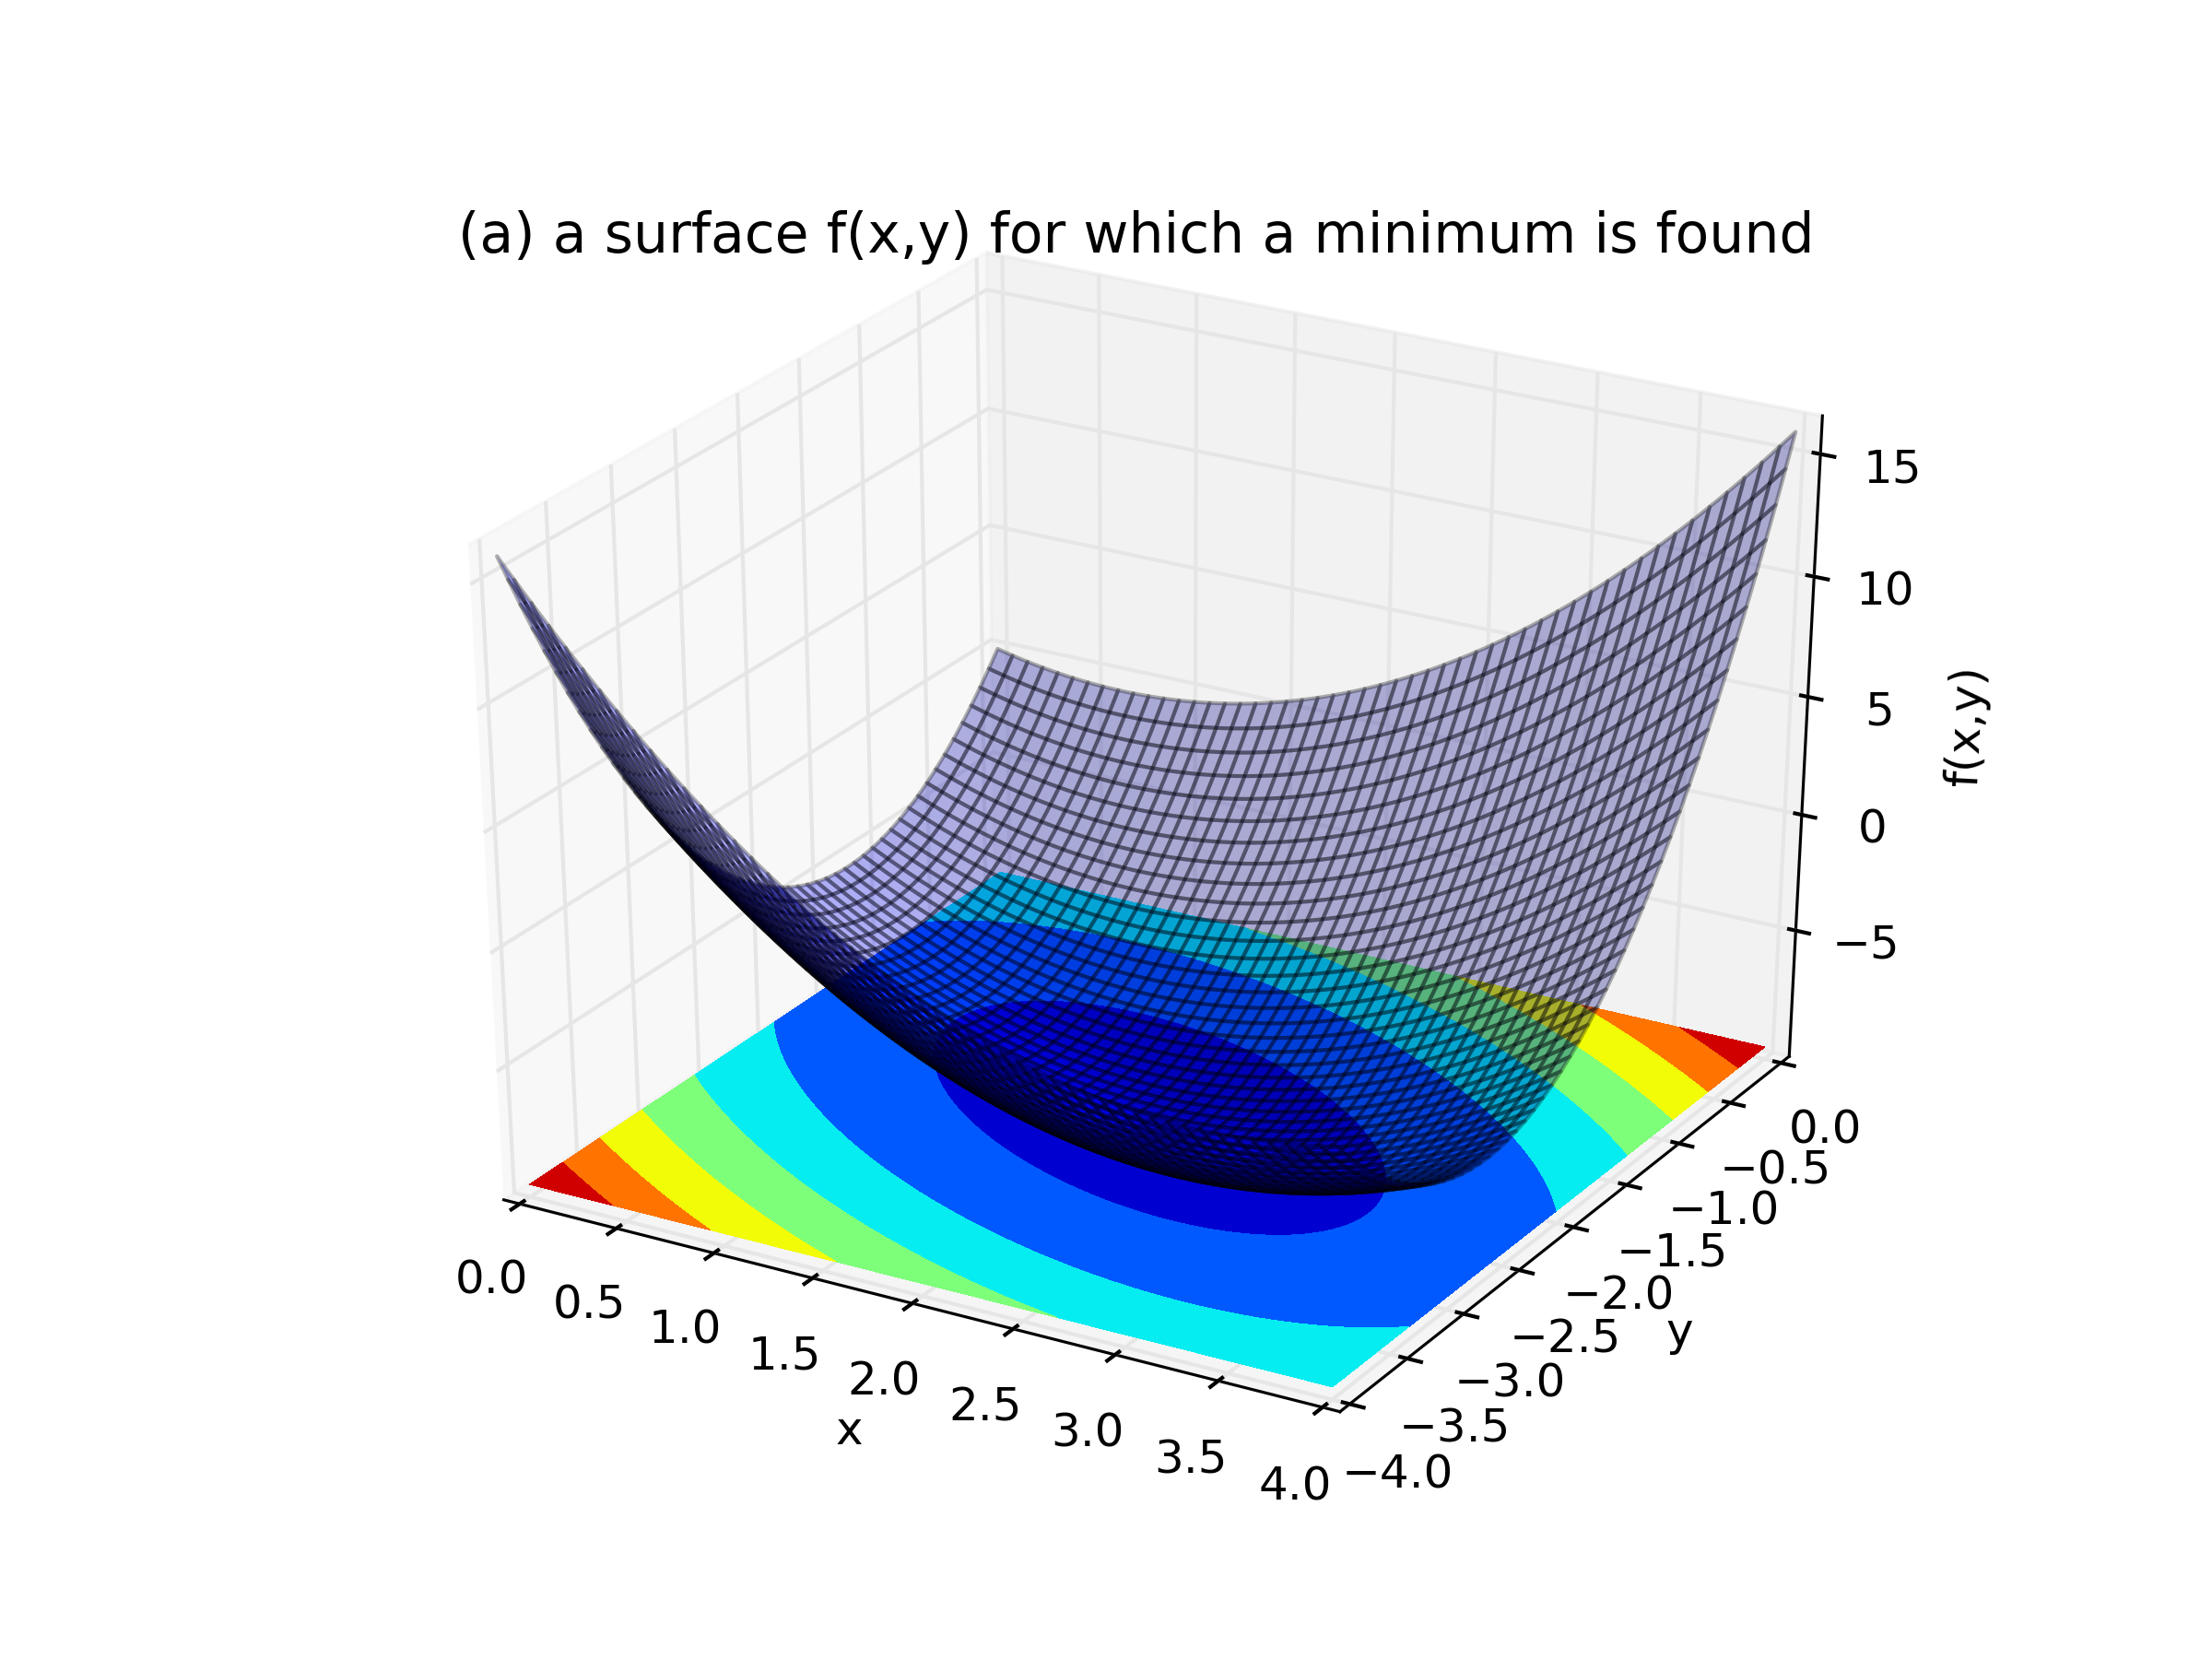
\includegraphics[width=\textwidth]{fig1}
        \caption{A plot of the surface
            $f = \rfrac{3}{2}x_1^2 + 2x_1 x_2 + 3x_2^2 - 2x_1 + 8x_2$,
          showing a contour plot in the xy-plane.
          A recreation of Fig 2.1(a) from the text.} 
    \end{figure}

    The script \texttt{p2b.py} contains the actual algorithm used to find the
    solution (whereas \texttt{luke\_Wukmer\_HW1\_Prob2.py} is restricted in
    scope to generating the necessary figures). The brunt of the algorithm is
    essentially a faithful porting of the algorithm described in pp.42-3 of the
    text. When run by itself, it provides about gradient descent convergence
    (run in this particular case will tolerance \texttt{10e-6}):
    
    \begin{small}
    \begin{verbatim}
    wukm@zoo ~/573/hw1 % p2b.py
    converged in 9 iterations.
    step 0: f(1	,-0.2)	= -2.38
    step 1: f(0.9041163435498009	,-1.6062936279362545)	= -8.596457152247144
    step 2: f(1.8158080581710858	,-1.6684544745739032)	= -9.741478714823582
    step 3: f(1.798147051701616	,-1.927482457095344)	= -9.95238245848541
    step 4: f(1.9660733282096614	,-1.9389319809148695)	= -9.991229231827678
    step 5: f(1.9628203117633845	,-1.9866428520181425)	= -9.998384495162707
    step 6: f(1.9937509872961738	,-1.9887517633391165)	= -9.999702437023984
    step 7: f(1.9931518048176313	,-1.9975397215892408)	= -9.999945191358062
    step 8: f(1.9988489831096707	,-1.9979281675378637)	= -9.99998990469924
    step 9: f(1.9987386189780325	,-1.9995468337889295)	= -9.99999814052855
    \end{verbatim} 
    \end{small}
    
    A visualization of this convergence to the solution is shown in Fig 2
    (below).  Note that by the nature of the gradient descent algorithm, each
    segment is exactly perpindicular to the level curve passing through each
    $f(x_i)$.

    \begin{figure}[t]
        \centering
        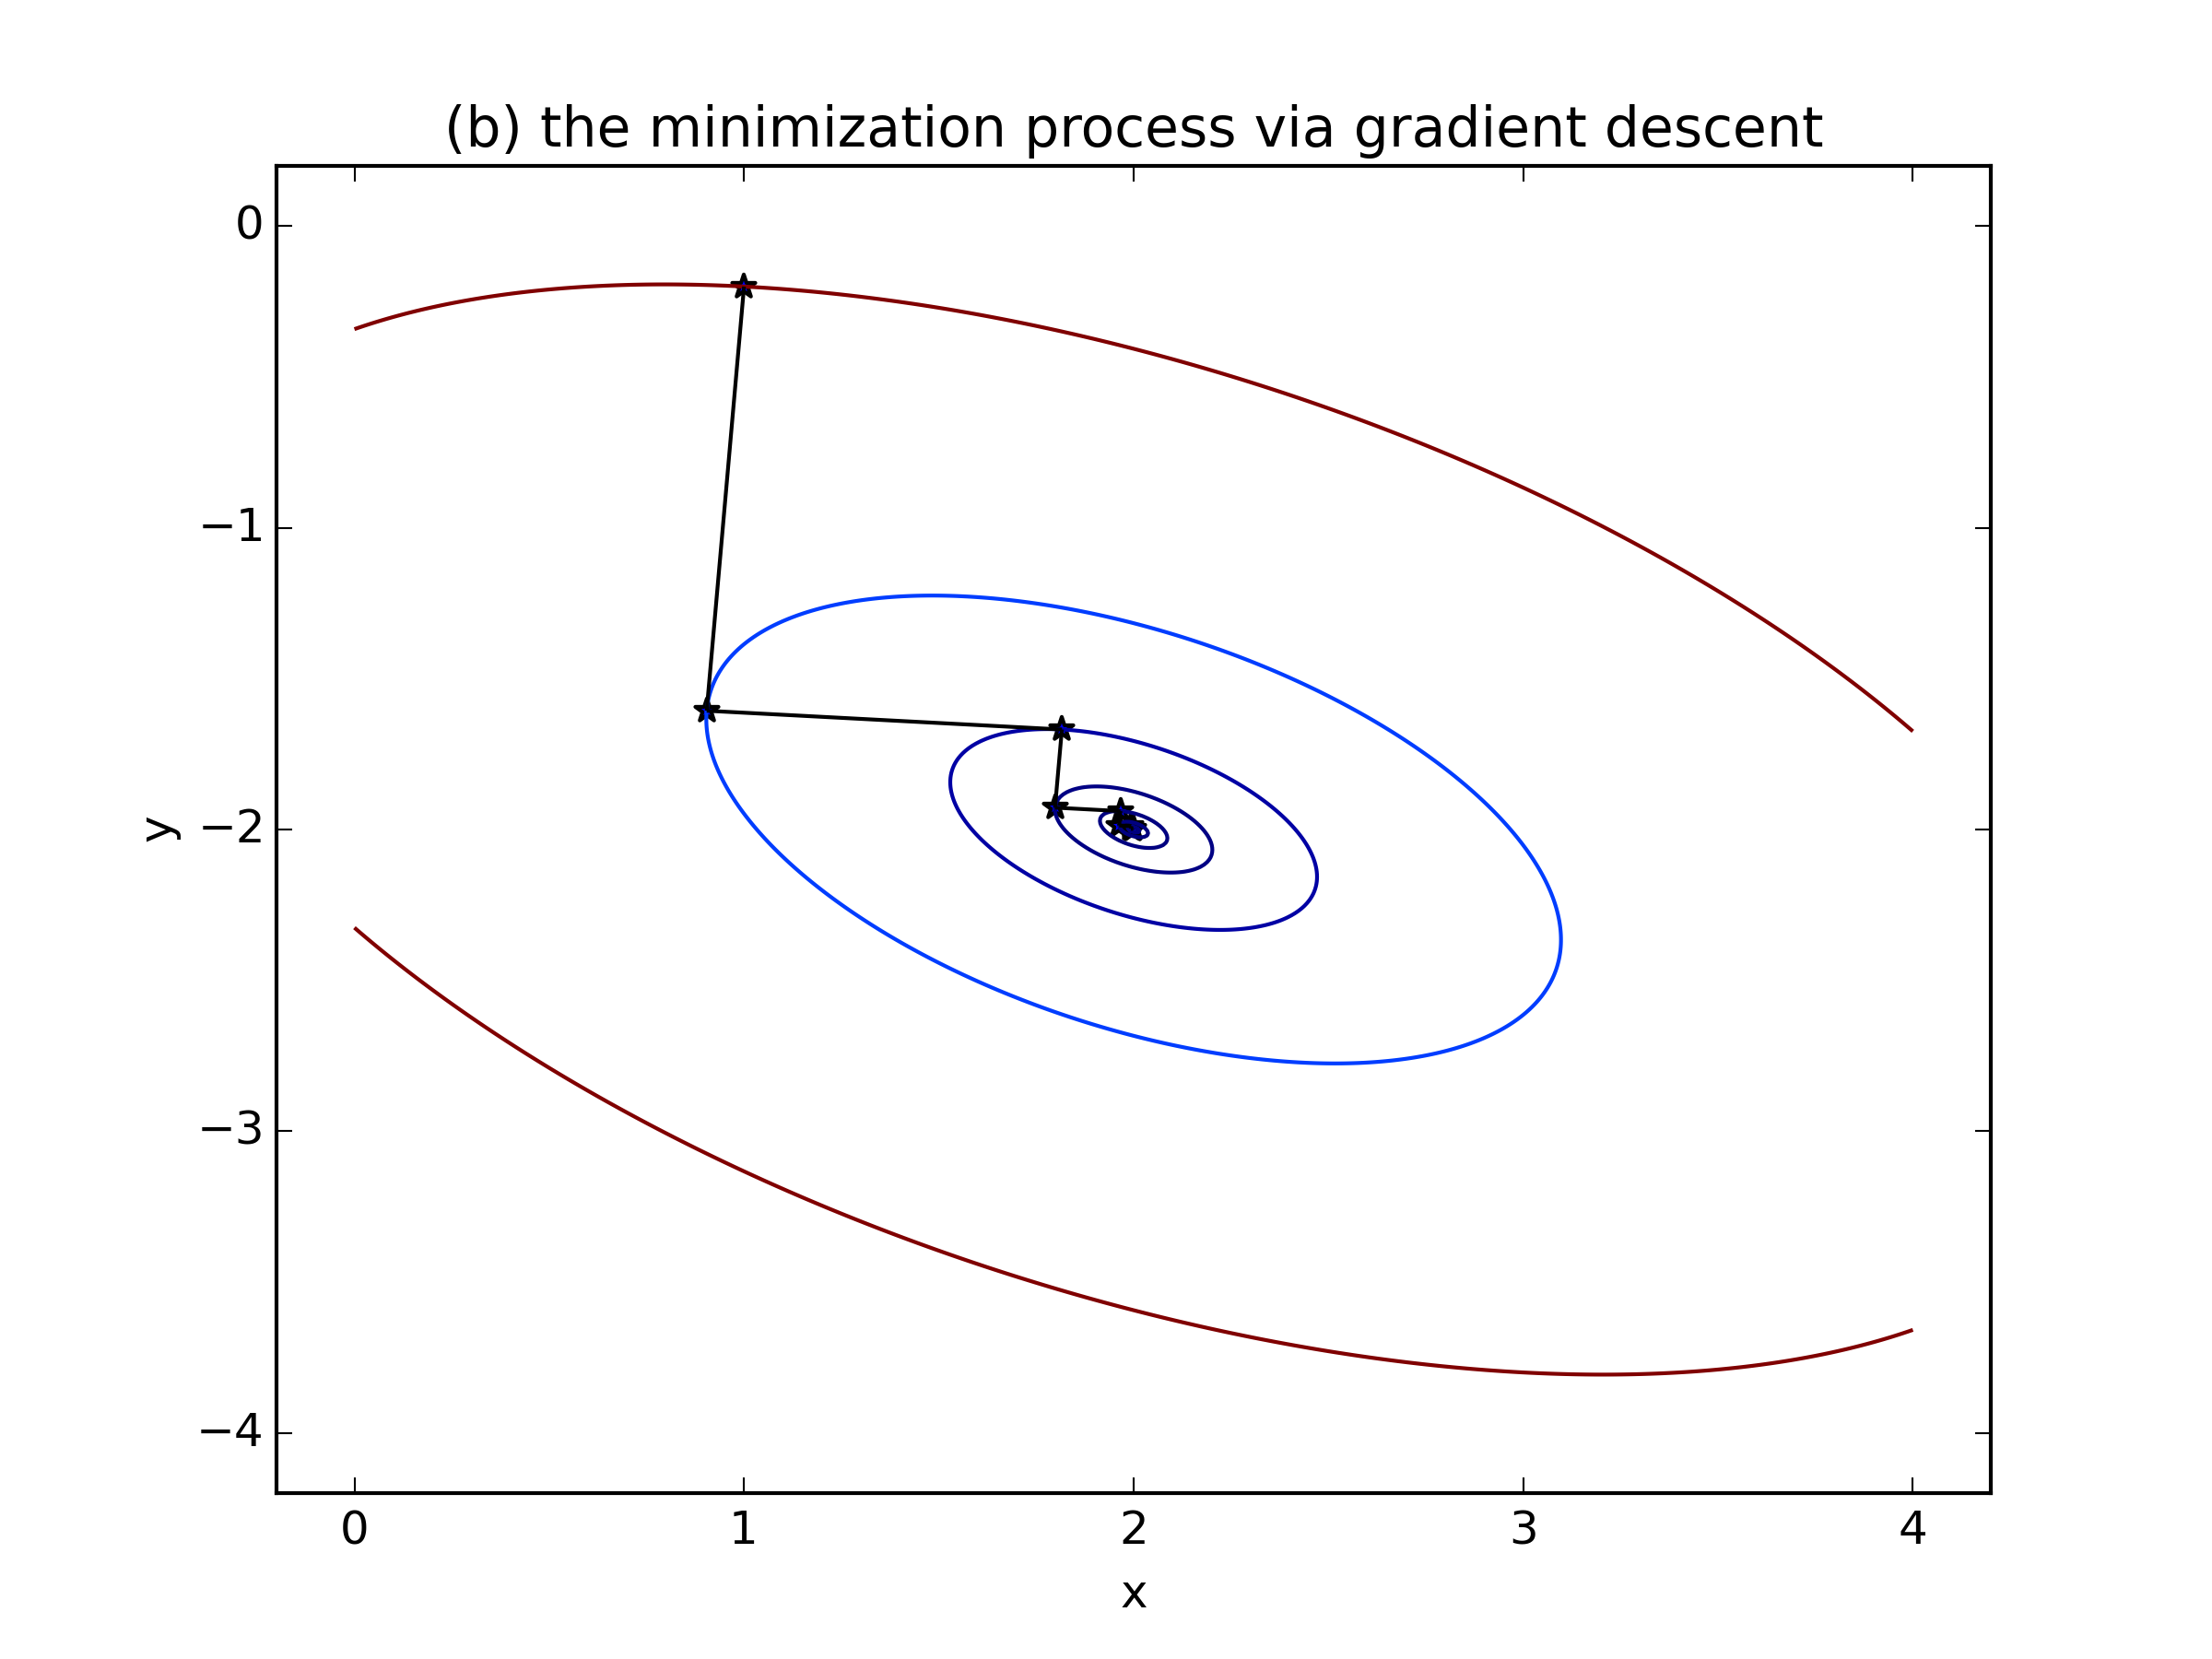
\includegraphics[width=\textwidth]{fig2}
        \caption{A visualization of gradient descent performed on the surface
            in Fig. 1. Each star represents the estimated $x_i$ at the
            $i^{\text{th}}$ iteration. Contours here pass through all points
            $(x,y) \st f(x,y) = f(x_i).$
        }
    \end{figure}
\end{prob}

\hrulefill
\clearpage
%%% PROBLEM 3
\begin{prob}

    Refer to \texttt{steepest\_descent.py} and \texttt{luke\_Wukmer\_HW1\_Prob3.py}.
    For the given $5\times5$ system, the following output was generated:

\begin{verbatim}
wukm@zoo ~/573/hw1 % python luke_Wukmer_HW1_Prob3.py
terminated in 110 iterations (out of M=10000) with tolerance eps=1e-09
x =  [[ 1. -2.  3. -2.  1.]]
 \end{verbatim}

 which is easily verified as the solution of the system.
\end{prob}
\hrulefill

%%% PROBLEM 4
\begin{prob}
The conjugate gradient method for solving a linear system was implemented and tested on a given linear system.
Refer to the files \texttt{luke\_Wukmer\_HW1\_Prob4.py} and \texttt{conjugate\_gradient.py}.

\subsection*{(a)}

A conjugate gradient method for solving the system $Ax=b$ where A is symmetric
positive definite was implemented in \texttt{conjugate\_gradient.py}. The
function \texttt{conjugate\_gradient(A, b, [...])} first checks that A is an
SPD matrix, and then searches for a solution via conjugate gradient method.
When this file is run by itself, a random $100\times100$ SPD matrix
and $100\times1$ b vector is generated and tested with tolerance $ε=10e-10$.
Here is a sample test:

\begin{verbatim}
wukm@zoo ~/573/hw1 % python conjugate_gradient.py
tolerance reached!
finished in 162 iterations
|| b - Ax || =  6.94833183485e-10
\end{verbatim}

Of course, theoretically this should have converged within 100 iterations, but
we can attribute this discrepancy to unnecessarily high tolerance used.

Refer to \texttt{util.py} for the method of generating random SPD matrices,
which involves creating a symmetric matrix from a uniformly random initial
matrix and assuring that it is diagonally dominant.

\subsection*{(b)}

The conjugate gradient method detailed above is now tested on a particular system with a known solution. A Hilbert matrix $H$ and a corresponding $b$ vector are given as:
\[
        H \in \R^{n\times n} \st H_{ij} = \left(i + j - 1\right)^{-1} \quad , \quad
        b \in \R^{n\times 1} \st b_i = \frac{1}{3} \sum_{j=1}^n a_{ij}
    \]

    Clearly the solution to the system $Hx=b$ should be $x^{\bigstar} = \frac{1}{3}(1, 1, \cdots, 1)^T$.

A sample running with parameters \texttt{N=15, $\epsilon$=10e-12} finds the
solution as expected, and within the theoretical limit of iterations. Since we
know the true solution $x^{\bigstar}$ we can calculate the error in the found solution
directly:

\begin{verbatim}
wukm@zoo ~/573/hw1 % python luke_Wukmer_HW1_Prob4.py
running CG on a 15-by-15 Hilbert matrix with tolerance 1e-11
tolerance reached!
finished in 13 iterations
x =
 [[ 0.33333332  0.33333374  0.33332895  0.33335053  0.33330938  0.3333307
   0.33335197  0.33334662  0.33332767  0.33331508  0.33331875  0.33333558
   0.33335266  0.33335179  0.33331325]]
|| x - x* || =  5.58600900773e-05
\end{verbatim}

In fact, the high conditioning number of the Hilbert matrix doesn't seem to prevent this method succeeding for even higher dimensions:

\begin{verbatim}
wukm@zoo ~/573/hw1 % python luke_Wukmer_HW1_Prob4.py
running CG on a 150-by-150 Hilbert matrix with tolerance 1e-11
tolerance reached!
finished in 27 iterations
x = (output suppressed)
|| x - x* || =  0.000371820210278
\end{verbatim}

As shown, this implementation of conjugate gradient returns reasonably accurate
solutions to randomly generated linear systems, as well as returning an accurate solution
to the problem-at-hand.
\end{prob}
\hrulefill

\subsection*{\textsc{TODO}}
  \begin{itemize}
    \item Investigate behavior of \texttt{util.random\_spd()} function
    \item Investigate use of more appropriate tolerances $(\epsilon)$ so as to
          not introduce unnecessary error
    \item Clean up \texttt{luke\_Wukmer\_HW1\_Prob2.py} (see docstring)
  \end{itemize}
\end{document}
